\section{Evaluation}
\label{exp}
%We evaluate the implementations on two platforms. The first is the  NVIDIA Tesla K40m, which facilitates 2880 FP32 cores with a 64KB L1 cache and shared memory. The host machine has a 2.40GHz Intel Xeon E5-2620 CPU with 128GB memory and Linux kernel v4.19.85. 
We evaluate the implementations on the NVIDIA RTX 2080 Ti, which facilitates 4350 FP32 cores and 4350 INT32 cores with a 96KB L1 cache and shared memory. The host machine has a 2.30GHz Intel Xeon E5-2697
CPU with 252GB memory and Linux kernel v4.15.0. The platform is shipped with the CUDA Toolkit v10.2. We use the following state-of-the-art image and convolution libraries for comparison:
\begin{itemize}
  \item cuDNN, version 7.6.4. cuDNN is a state-of-the-art convolution implementation that supports 2D and depth-wise convolutions on GPU.
      Moreover, cuDNN can execute GEMM-, FFT- and Winograd-based convolutions.
  \item ArrayFire \cite{Yalamanchili2015}, version 3.6.4. ArrayFire is a popular image and signal processing library. This library implements single-channel 2D convolutions on GPU. ArrayFire uses Just In Time compiling for standard arithmetic operations; thus, the first run of an ArrayFire application takes longer than the second run.
      In the experiment, we run ArrayFire twice in each test and record the second runtime.
  \item NVIDIA Performance Primitives (NPP). NPP is an image and signal processing library. We use NPP for single-channel 2D convolutions only.
  \item GEMM-im2col (im2col). We extract the implementation of the im2col from Caffe \cite{jia2014caffe} and take it as a baseline for the single-channel 2D convolution.
  \item Direct implementation of depth-wise convolution. We implement a direct depth-wise convolution without using the proposed reuse algorithms. We take this implementation as a baseline for depth-wise convolution.

\end{itemize}

%After years of updating, cuDNN has integrated seven widely used convolution algorithms. We use the Therefore, cuDNN provides an option that uses heuristics to find the most suitable algorithm for a convolution. We set the option to $PREFER\_FASTEST$ (the exact option can be found at
%\cite{CUDAtoolkit}); that is, we prefer to use the fastest algorithm regardless of the memory capacity. However, the algorithm selected by the heuristic is not always the fastest. Therefore, we use two types of runtime for cuDNN. One is the real fastest runtime among the seven algorithms and the other is the heuristically fastest runtime. For 2D convolutions, we use the real fastest runtime because two types of runtime are the same.

%Our implementations of convolution use only a small part of shared memory and mainly relay on GPU L1 cache. Therefore we employ $cudaDeviceSetCacheConfig$ function to set GPU cache policy with arguments $cudaFuncCachePreferL1$ for our convolutions.
We run each test case ten times and report the averaged running time. All data are 32-bit float data type and organized as 4D tensors $(N,C,H,$ and $W)$. For
now, we test single-channel 2D and depth-wise convolutions for the filters of size $3 \times 3$ and $5 \times 5$, because small filters are commonly used in applications. The results for the single-channel 2D convolution are presented first in the subsequent section, followed by that for the depth-wise convolution.

\subsection{Single-channel 2D Convolution}
\begin{figure*}
\centering
%\subfloat[Speedups for the filter of size $3 \times 3$ on Tesla K40m.]{\includegraphics[width=\columnwidth,height=6cm]{./figure/2d_norm_f3.eps}
	%\label{fig:2druntimef3c1}}
%\hspace{0em}
%\subfloat[Speedups for the filter of size $5 \times 5$ on Tesla K40m.]{\includegraphics[width=\columnwidth,height=6cm]{./figure/2d_norm_f5.eps}
	%\label{fig:2druntimef5c1}}

\subfloat[Speedups for the filter of size $3 \times 3$.]{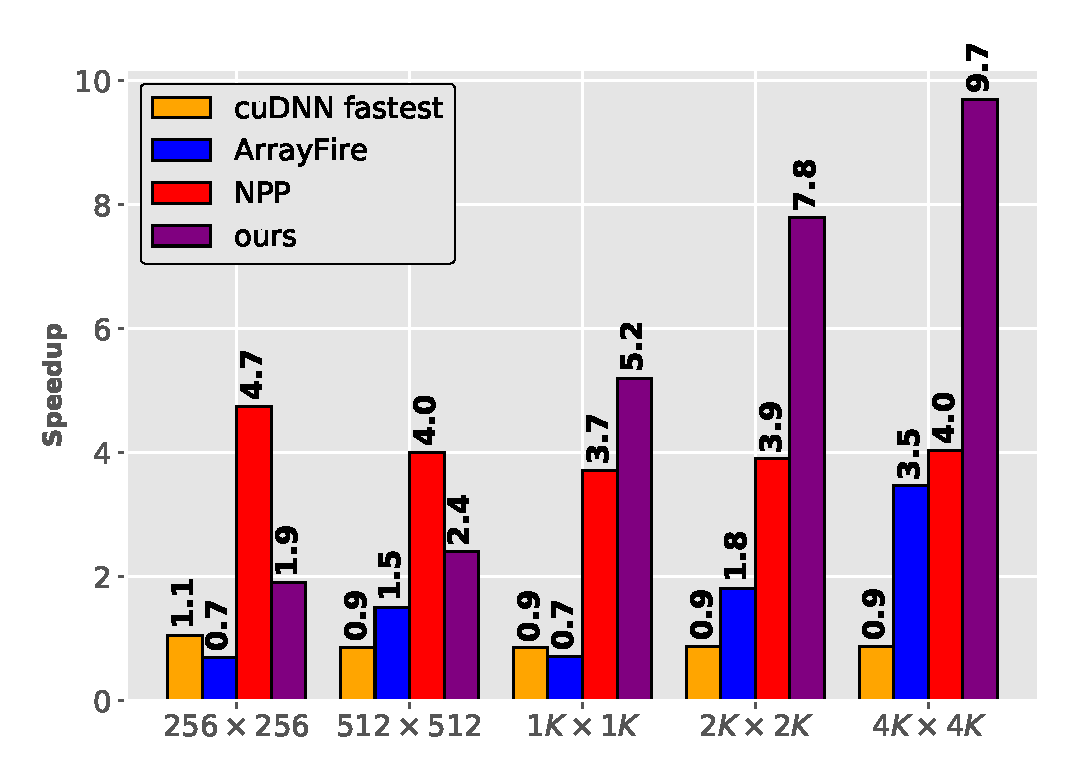
\includegraphics[width=\columnwidth,height=6cm]{./figure/2d_conv_f3.eps}
	\label{fig:2druntimef3c12080}}
\hspace{0em}
\subfloat[Speedups for the filter of size $5 \times 5$.]{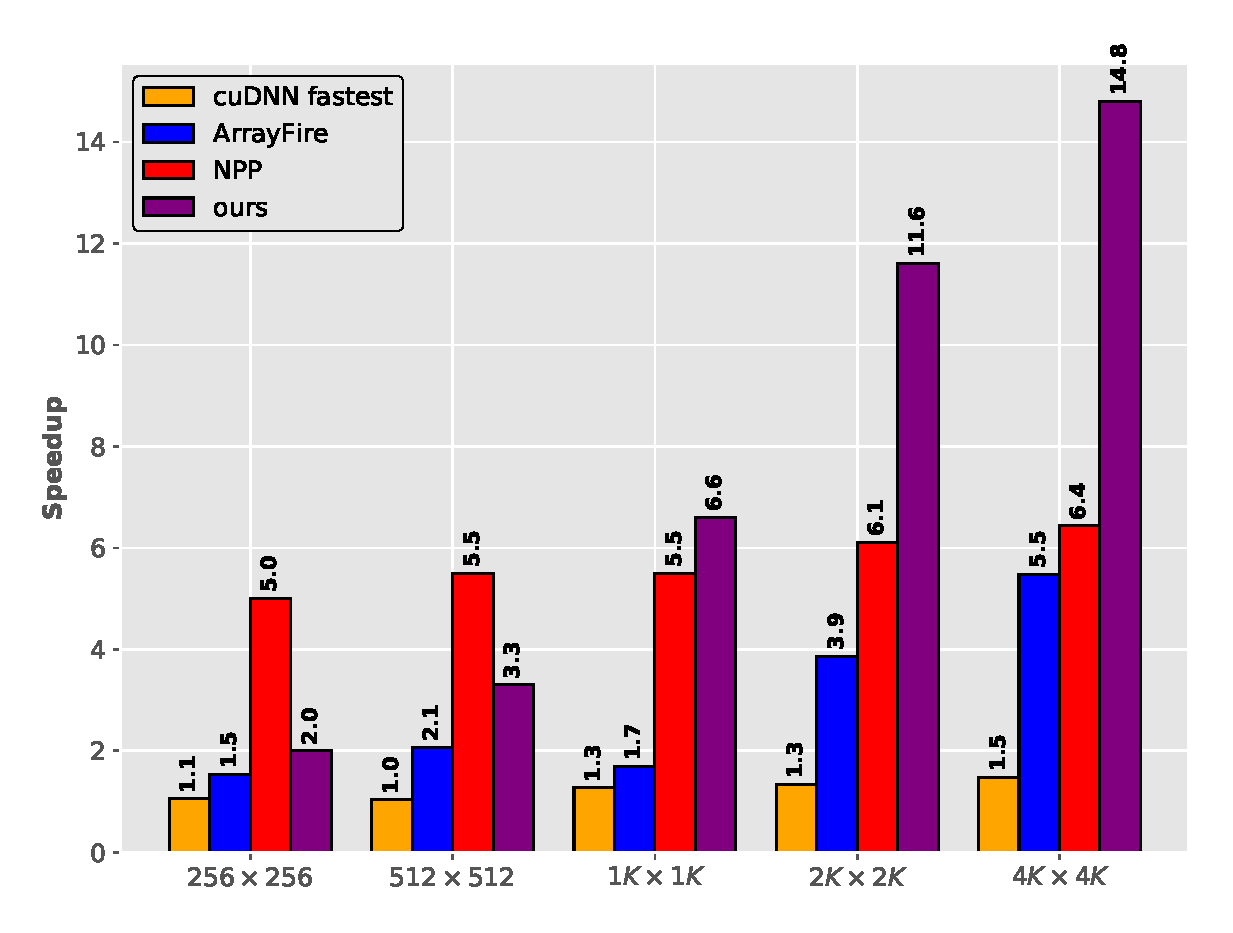
\includegraphics[width=\columnwidth,height=6cm]{./figure/2d_conv_f5.eps}
	\label{fig:2druntimef5c12080}}
	
\caption{Speedups of single-channel 2D convolution of four implementations over im2col on RTX 2080Ti.}
\label{fig:2druntime}
\end{figure*}

%\begin{table*}[]
%\caption{Summation of memory transactions on each type of memory, including global memory, texture memory and shared memory.}
%\label{tab:2dmemtrans}
%\begin{tabular}{c|ccccc|ccccc}
%\hline
%\multicolumn{1}{l|}{}                & \multicolumn{5}{c|}{Filter size $3 \times 3$}                                                & \multicolumn{5}{c}{Filter size $5 \times 5$}                                                \\ \hline
% & $256 * 256$      & $512 * 512$      & $1K * 1K$        & $2K * 2K$        & $4K * 4K$        & $256 * 256$      & $512 * 512$      & $1K * 1K$        & $2K * 2K$        & $4K * 4K$        \\ \hline
%cuDNN                                                  & 6.0E+05          & 2.4E+06          & 9.7E+06          & 3.9E+07          & 1.5E+08          & 1.4E+06          & 5.6E+06          & 2.2E+07          & 8.9E+07          & 3.6E+08          \\
% im2col & 1.1E+05          & 4.4E+05          & 4.4E+05          & 7.0E+06          & 2.8E+07          & 2.3E+05          & 9.3E+05          & 3.7E+06          & 1.5E+07          & 6.0E+07          \\
%im2row & 1.1E+05          & 4.4E+05          & 4.4E+05          & 7.0E+06          & 2.8E+07          & 2.3E+05          & 9.3E+05          & 3.7E+06          & 1.5E+07          & 6.0E+07          \\
%ArrayFire                                              & 4.9E+04          & 2.0E+05          & 7.9E+05          & 3.2E+06          & 1.3E+07          & 1.1E+05          & 4.2E+05          & 1.7E+06          & 6.8E+06          & 2.7E+07          \\
%NPP                                                    & 6.0E+04          & 2.4E+05          & 9.6E+05          & 3.8E+06          & 1.5E+07          & 1.3E+05          & 5.2E+05          & 2.1E+06          & 8.3E+06          & 3.3E+07          \\
%Ours                                                   & \textbf{7.5E+03} & \textbf{2.7E+04} & \textbf{1.1E+05} & \textbf{4.2E+05} & \textbf{1.6E+06} & \textbf{1.0E+04} & \textbf{3.3E+04} & \textbf{1.3E+05} & \textbf{4.9E+05} & \textbf{1.9E+06} \\ \hline
%\end{tabular}
%\end{table*}

This section presents the performance of the single-channel 2D convolution obtained from five implementations, including cuDNN, im2col,  ArrayFire,
NPP and the proposed method. We evaluate the five implementations with the image size ($I_H \times I_W$) ranging from $256 \times 256$ to $4K \times 4K$, $I_N=F_N=1$ and $I_C=F_C=1$. 
%We first present the speedups of four implementation over im2col in Figure \ref{fig:2druntime}. Then we show the effectiveness of our implementation on reducing the number of memory transactions in Table \ref{tab:2dmemtrans}.

Figure \ref{fig:2druntime} presents the speedups of cuDNN, ArrayFire, NPP and our implementation over im2col. The results show that cuDNN is not suitable for single-channel 2D convolutions in contrast to ArrayFire, NPP and the proposed method. The average speedups of cuDNN, ArrayFire, NPP and ours over im2col are 1.09$\times$, 2.2$\times$, 4.9$\times$ and 6.5$\times$, respectively. Our implementation exhibits superior performance over other implementations. Our implementation of the single-channel 2D convolution is derived from direct convolution. We use column (Algorithm \ref{algo:basic}, Algorithm \ref{algo:basic2}) and row reuse (Algorithm \ref{algo:rowreuse}) on direct convolution. Hence, the performance gains are mainly attributed to the reduction on the number of memory transactions.

%Figure \ref{fig:2druntimef3c1} and \ref{fig:2druntimef5c1} present the speedups on Tesla K40m in which the proposed method achieves the best results in nine cases out of ten. Our implementation is  slower than NPP when performing a $3 \times 3$ convolution on a $256 \times 256$ image. The average speedups of our implementation over ArrayFire and NPP on Tesla K40m are 2.1$\times$ and 2.9$\times$, respectively.
%Figure \ref{fig:2druntimef3c12080} and \ref{fig:2druntimef5c12080} show the speedups on RTX 2080 Ti, in which 
In all of ten test cases, the proposed implementation achieves the best results in six cases out of ten. NPP achieves the best results on small image sizes, whereas our implementation demonstrates the best results on large image sizes. We use \emph{nvidia compute} to collect memory profiles, including memory throughput and max bandwidth, of our implementation and NPP when convolving with a $3 \times 3$ filter. The results are shown in Figure \ref{fig:2dmemanaly}.

The average speedup of our implementation for the $5 \times 5$ filter is $7.7\times$, which is better than the speedup for the $3 \times 3$ filter, $5.4\times$. The key reason for this improvement is that, for the $3 \times 3$ filter, there is only one overlapped column and row on width and height dimensions. While for the $5 \times 5$ filter, there are four overlapped columns and rows, therefore column and row reuse algorithms can be used more efficiently compared with  that for the $3 \times 3$ filter.

We can see that as the input size increases, memory throughput and max bandwidth of our implementation exceeds that of NPP, the turning point ($1K \times 1K$ in Figure \ref{fig:2dmemanaly}) is the same as that of speedups in Figure \ref{fig:2druntimef3c12080}, which means that memory performance has a strong relation to the performance of single-channel 2D convolution. Next, we give a detailed analysis of why the memory throughput and max bandwidth of our implementation is low for small input sizes.

When performing single-channel 2D convolutions, only one filter are used to convolve with one single-channel input feature map, which requires much less computation than depth-wise convolutions. Therefore, the memory performance is a deciding factor to the runtime of the single-channel 2D convolution. The proposed row reuse algorithm performs better when a thread calculates more rows of output. However, the more rows each thread calculates, the less warps and thread blocks we can generate. Without enough warps issuing memory requests, the memory throughput and max bandwidth can reduce significantly, which can slow down our implementation. As the input size increases, we can allocate more thread blocks and more warps per thread block. With enough memory requests and reduction on redundant memory transactions, we can increase the memory throughput and max bandwidth, and thus improve the performance of our implementation.

%We use \emph{nvprof} to collect the number of memory transactions for the different types of memories. The GPU global memory is used to store the input data in im2col, im2row, ArrayFire and our implementation. NPP and cuDNN utilize texture memory to store input data, whereas shared memory is normally used to store filter data. Therefore, we sum up the number of read transactions of the three memory types and report the results in Table
%\ref{tab:2dmemtrans}. To save space, we only show the result of the memory transactions collected on Tesla K40m because the result on RTX 2080 Ti exhibits a similar trend.

\begin{figure}
\centering

\subfloat[Memory throughput for the filter of size $3 \times 3$.]{\includegraphics[width=\columnwidth,height=6cm]{./figure/2dmemthroughput.eps}
	\label{fig:2dmemthr}}
\hspace{0em}
\subfloat[Max bandwidth for the filter of size $3 \times 3$.]{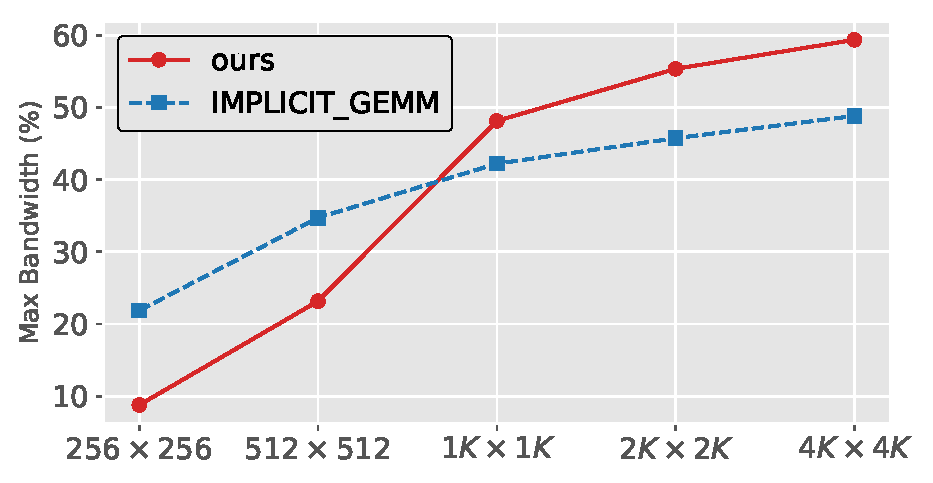
\includegraphics[width=\columnwidth,height=6cm]{./figure/2dmembandwidth.eps}
	\label{fig:2dmaxband}}
	
\caption{Memory analysis of NPP and our implementation for the filter of size $3 \times 3$.}
\label{fig:2dmemanaly}
\end{figure}

%The results in Table \ref{tab:2dmemtrans} verify that our optimization algorithms significantly reduce the number of memory transactions.
%Compared with ArrayFire and NPP, which are well optimized for 2D convolutions, our implementation can respectively reduce the memory transactions by a factor of 10.2 and 12.3 on average.


% Please add the following required packages to your document preamble:
% \usepackage{multirow}


%\begin{table*}[]
%\caption{2d speedup}
%\label{tab:2dspeedup}
%\begin{tabular}{c|ccccc|ccccc}
%\hline
%\multicolumn{1}{c}{}&\multicolumn{5}{c}{$F_H*F_W= 3*3$} &\multicolumn{5}{c}{$F_H*F_W= 5*5$}\\
%\hline
%           & 256*256&512*512&1K*1K&2K*2K&4K*4K&256*256&512*512&1K*1K&2K*2K&4K*4K\\
%\hline
%cuDNN      & 1.91 & 3.74 & 5.69 & 8.07 & 7.72     & 2.86 & 4.86 & 6.08 & 7.40 & 9.20  \\
%im2col     & 1.52 & 3.25 & 5.25 & 7.56 & 7.24     & 2.34 & 4.20 & 5.37 & 6.88 & 8.38  \\
%im2row     & 1.55 & 3.25 & 5.20 & 7.50 & 7.19     & 2.34 & 4.15 & 5.32 & 6.83 & 8.32  \\
%ArrayFire  & 1.23 & 3.67 & 2.59 & 2.37 & 1.95     & 1.40 & 3.12 & 1.73 & 1.43 & 1.57  \\
%NPP        & 0.68 & 1.40 & 2.21 & 3.15 & 3.03     & 1.52 & 2.91 & 3.79 & 4.66 & 5.82 \\
%\hline
%\end{tabular}
%\end{table*}
In summary, our optimization algorithms can significantly reduce the number of memory transactions and improve the performance of single-channel 2D
convolutions. Compared with state-of-the-art image processing libraries, NPP, our implementation achieves average speedups of 1.3$\times$ and 1.28$\times$ for the $3 \times 3$ and $5 \times 5$ filters, respectively.

\subsection{Depth-wise Convolution}
\label{3dconvexp}

\begin{table}[]
\caption{Configurations of 3D convolution}
\label{tab:3dconvconfigs}
\centering
\begin{tabular}{c|ccccc}
\hline
& $I_N$ & $I_C$ & $I_H \times I_W$ &  $F_H \times F_W$ \\
\hline
CONV1 & 512  & 32    & 112*112 & $3 \times 3$, $5 \times 5$  \\
CONV2 & 512  & 96    & 112*112  &$3 \times 3$, $5 \times 5$   \\
CONV3 & 512  & 144   & 56*56  &$3 \times 3$, $5 \times 5$    \\
CONV4 & 512  & 160    & 56*56  &$3 \times 3$, $5 \times 5$    \\
CONV5 & 512  & 192   & 28*28  &$3 \times 3$, $5 \times 5$    \\
CONV6 & 512  & 240   & 28*28  &$3 \times 3$, $5 \times 5$    \\
CONV7 & 512  & 256   & 28*28  &$3 \times 3$, $5 \times 5$    \\
CONV8 & 512  & 384   & 14*14  &$3 \times 3$, $5 \times 5$    \\
CONV9 & 512  & 480   & 14*14  &$3 \times 3$, $5 \times 5$    \\
CONV10 & 512  & 672  & 14*14 &$3 \times 3$, $5 \times 5$     \\
CONV11 & 512  &672  & 7*7 & $3 \times 3$, $5 \times 5$      \\
CONV12 & 512  &960  & 7*7 & $3 \times 3$, $5 \times 5$      \\
CONV13 & 512  &1152  & 7*7 & $3 \times 3$, $5 \times 5$      \\
\hline
\end{tabular}
\end{table}

\begin{figure*}
\centering
		%\centering
		 %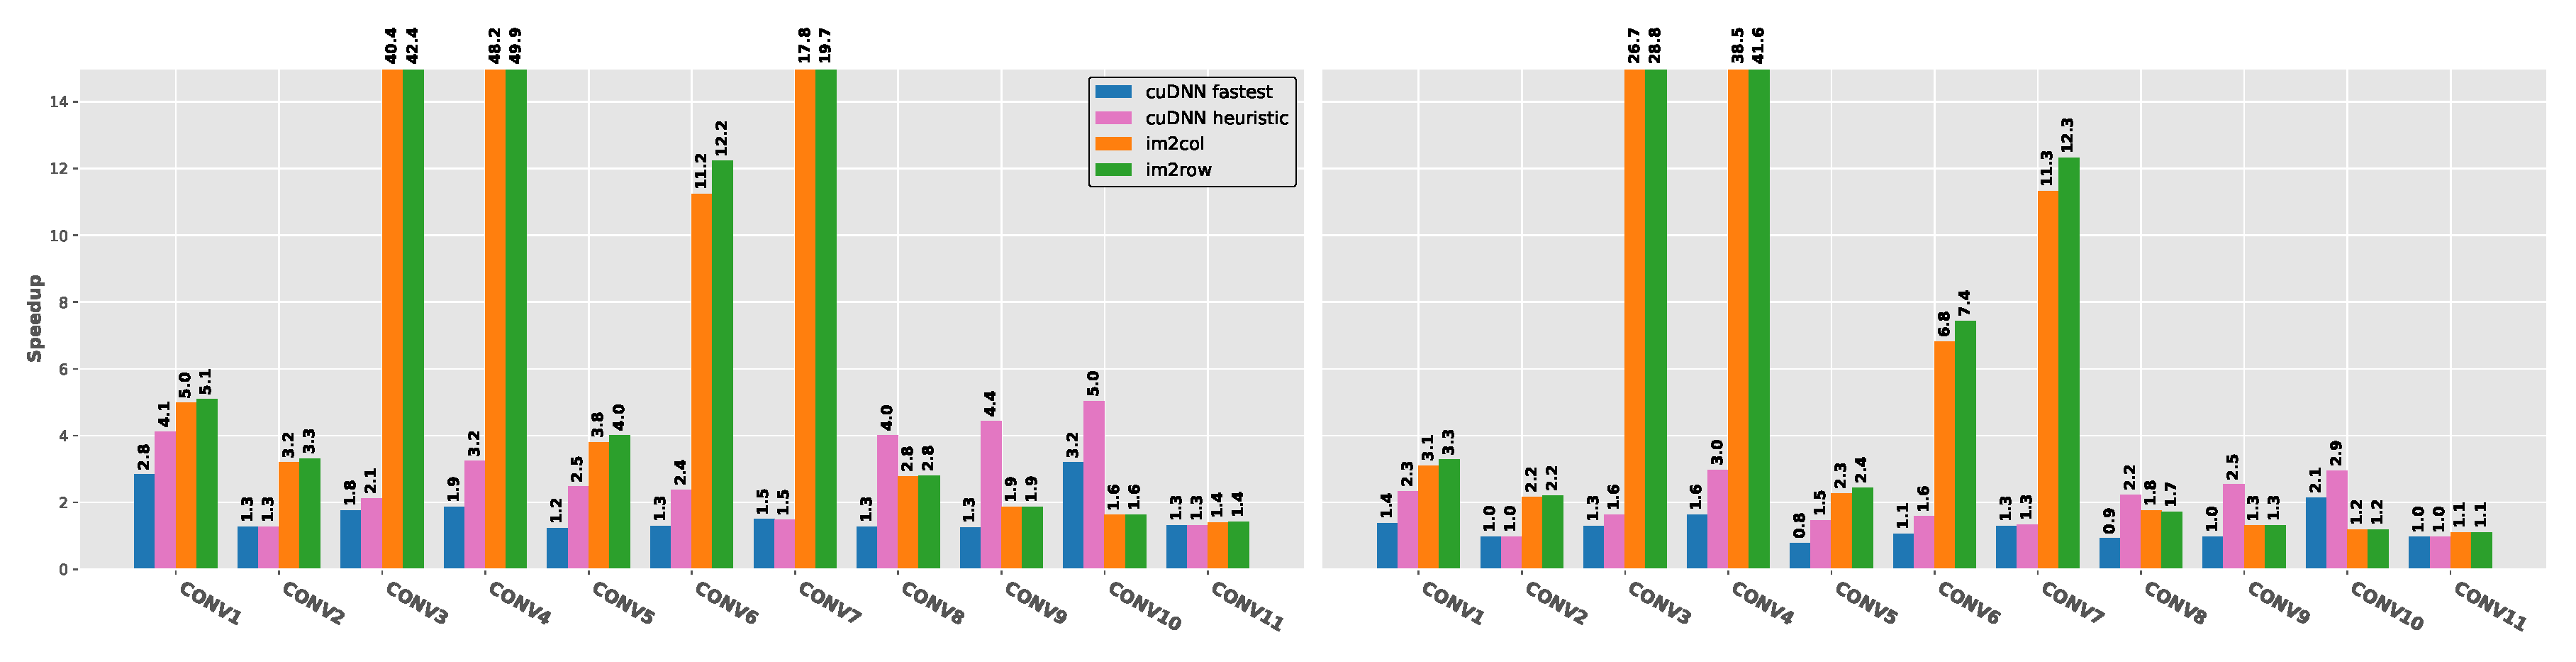
\includegraphics[width=18cm,height=5cm]{./figure/3d_norm_c1.eps}
		 %\caption{Normalized runtime of five implementations for 3D convolution. Left and right parts of the figure is for 3D convolutions with one and three input channels.}
		 %\label{fig:3druntime}
		
%\subfloat[Speedups on Tesla K40m, left is for one channel and right is for three channels.]{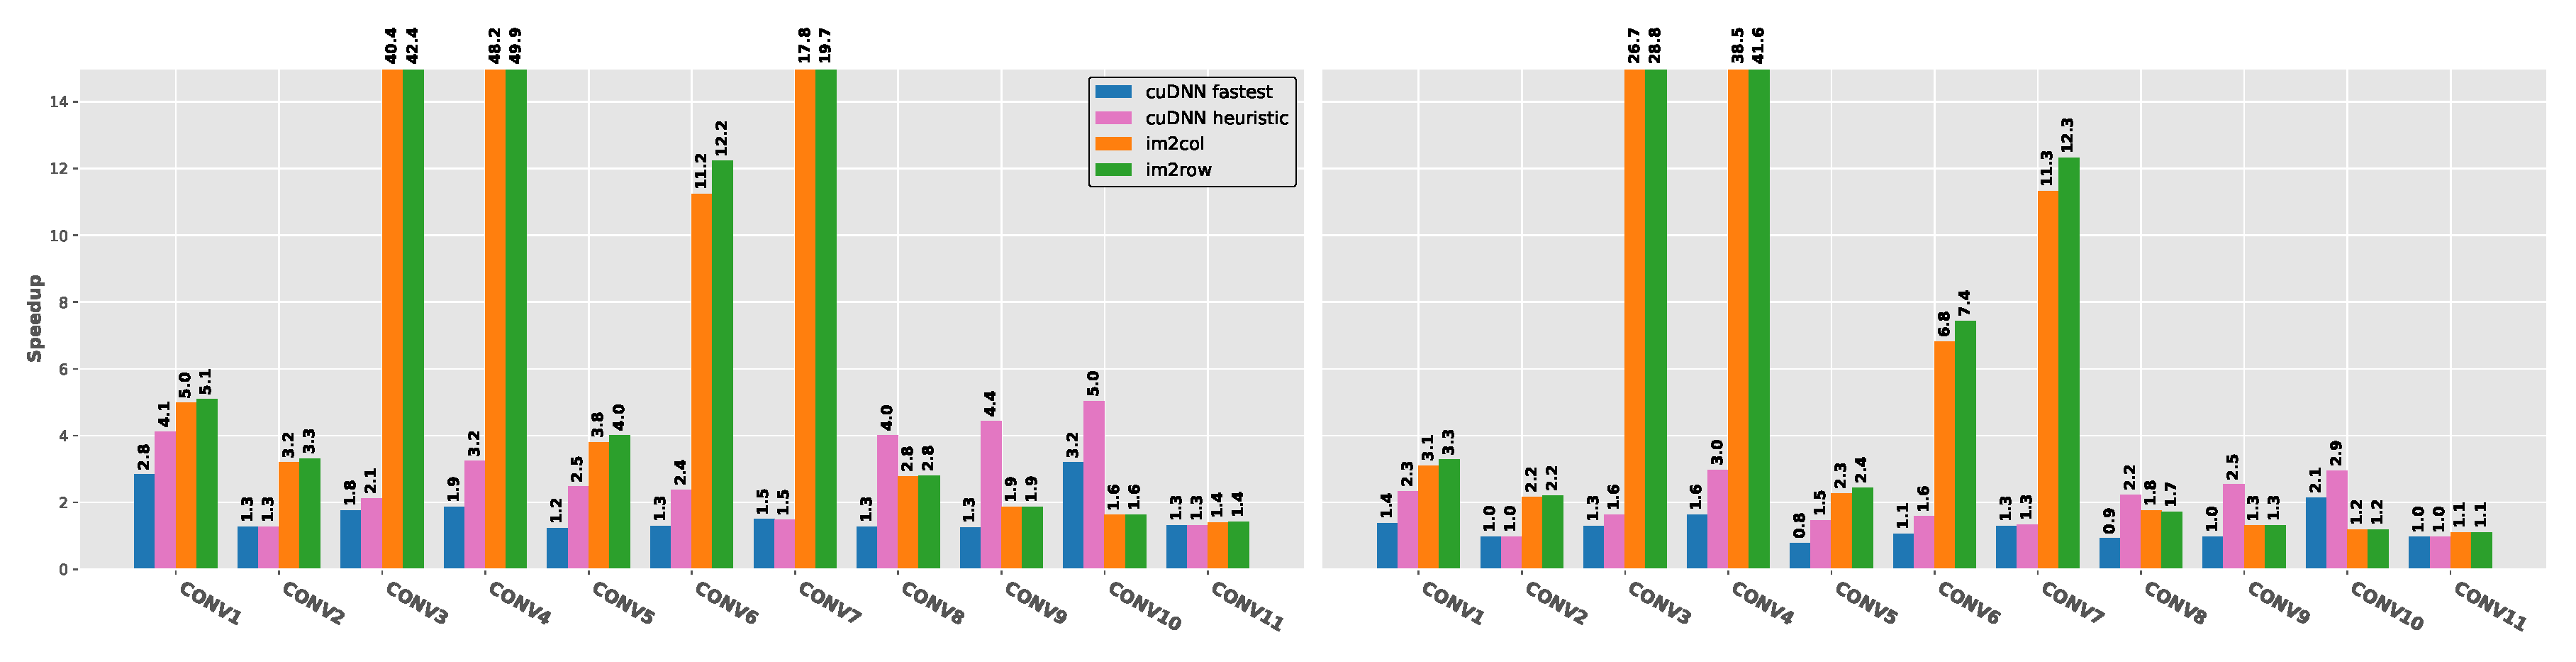
\includegraphics[width=18cm,height=5.7cm]{./figure/3d_norm_c1.eps}
%	\label{fig:3druntimeK40}}
	
\subfloat[Speedups for the filter of size $3 \times 3$.]{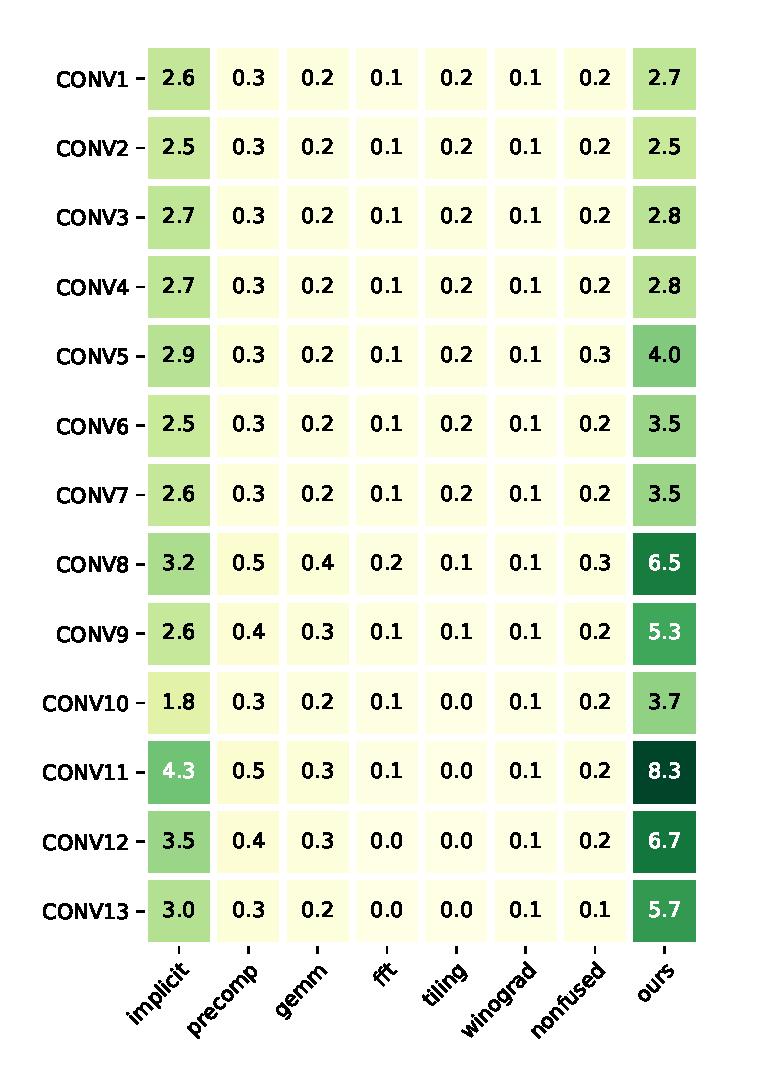
\includegraphics[width=\columnwidth,height=11cm]{./figure/depthwise_f3.eps}
	\label{fig:3druntime2080}}
\subfloat[Speedups for the filter of size $5 \times 5$.]{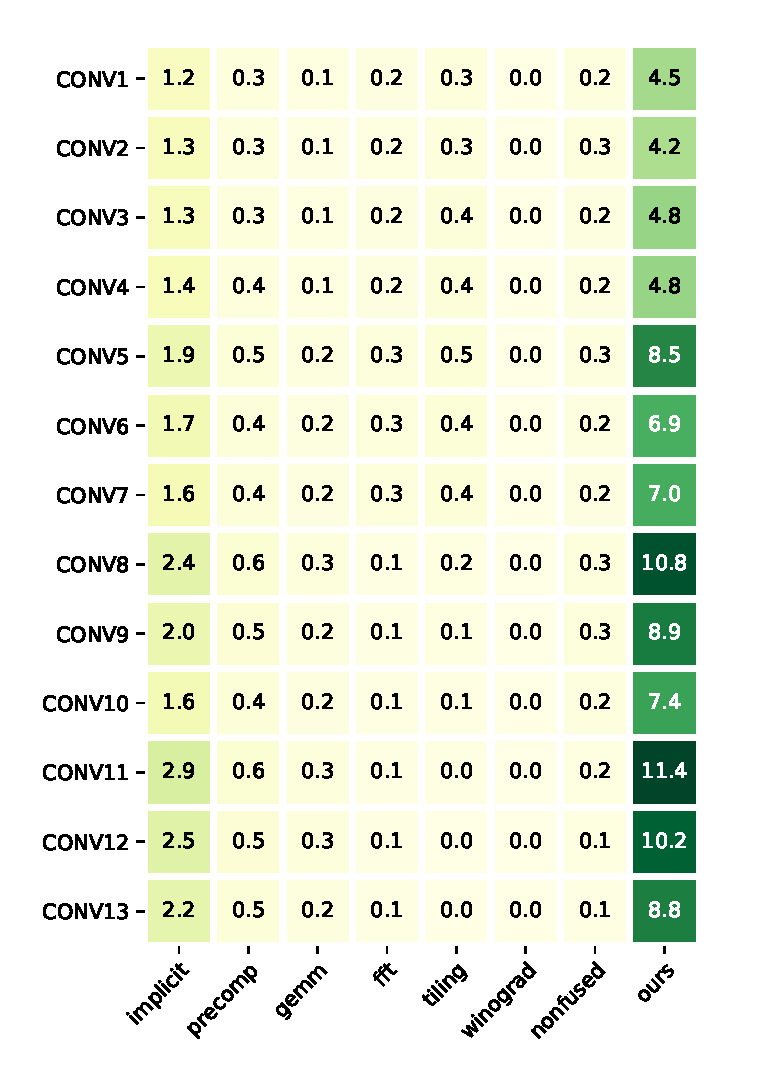
\includegraphics[width=\columnwidth,height=11cm]{./figure/depthwise_f5.eps}
	\label{fig:3druntime2080}}

\caption{Speedups of our implementation and seven cuDNN algorithms over the baseline implementation for the depth-wise convolution.}
\label{fig:3druntime}
\end{figure*}


%\begin{table*}[]
%\centering
%\caption{The number of memory transactions for 3D convolution. Data is collected on Tesla K40m.}
%\label{tab:3dtrans}
%\begin{tabular}{c|ccccc|ccccc}
%\hline
%\multicolumn{1}{l|}{} & \multicolumn{5}{c|}{$I_C=F_C=1$}                                                                                                                                                                                                                                                                  & \multicolumn{5}{c}{$I_C=F_C=3$}                                                                                                                                                                                                                                                                  \\ \hline
%    & \begin{tabular}[c]{@{}c@{}}cuDNN\\ fastest\end{tabular} & \begin{tabular}[c]{@{}c@{}}cuDNN\\ heuristic\end{tabular} & im2col & im2row & \begin{tabular}[c]{@{}c@{}}our 3D\\ conv\end{tabular} & \begin{tabular}[c]{@{}c@{}}cuDNN\\ fastest\end{tabular} & \begin{tabular}[c]{@{}c@{}}cuDNN\\ heuristic\end{tabular} & im2col & im2row & \begin{tabular}[c]{@{}c@{}}our 3D\\ conv\end{tabular} \\ \hline
%CONV1& 1.7E+06& 1.2E+07& 2.3E+06& 2.3E+06& \textbf{8.5E+05}& 3.9E+06& 1.3E+07& 5.5E+06& 5.5E+06& \textbf{2.4E+06}\\
%CONV2& 6.9E+06& 6.9E+06& 4.8E+06& 4.8E+06& \textbf{9.7E+05}& 1.6E+07& 1.6E+07& 1.2E+07& 1.2E+07& \textbf{2.9E+06}\\
%CONV3& 3.5E+05& 1.9E+05& 1.9E+05& 2.5E+05& \textbf{8.4E+04}& 9.5E+05& 5.2E+05& 5.2E+05& 6.8E+05& \textbf{2.5E+05}\\
%CONV4& 2.7E+05& 2.4E+05& 3.0E+05& 3.6E+05& \textbf{2.4E+04}& 7.4E+05& 6.4E+05& 8.0E+05& 9.8E+05& \textbf{7.3E+04}\\
%CONV5& 8.7E+06& 4.5E+06& 5.1E+06& 6.5E+06& \textbf{1.4E+06}& 1.2E+07& 1.2E+07& 1.4E+07& 1.8E+07& \textbf{4.1E+06}\\
%CONV6& 2.2E+06& 1.2E+06& 1.3E+06& 1.7E+06& \textbf{3.4E+05}& 5.9E+06& 3.2E+06& 3.6E+06& 4.6E+06& \textbf{1.0E+06}\\
%CONV7& 1.6E+06& 1.6E+06& 1.3E+06& 1.6E+06& \textbf{1.3E+05}& 1.7E+06& 4.3E+06& 3.6E+06& 4.5E+06& \textbf{3.9E+05}\\
%CONV8& 1.3E+07& 2.4E+07& 4.7E+06& 4.8E+06& \textbf{3.4E+06}& 3.0E+07& 2.9E+07& 1.1E+07& 1.2E+07& \textbf{9.8E+06}\\
%CONV9& 2.7E+07& 5.5E+07& 9.9E+06& 1.0E+07& \textbf{3.9E+06}& 6.5E+07& 5.7E+07& 2.4E+07& 2.4E+07& \textbf{1.2E+07}\\
%CONV10& 3.1E+07& 1.1E+08& 2.0E+07& 2.0E+07& \textbf{1.6E+07}& 7.1E+07& 1.2E+08& 5.0E+07& 5.1E+07& \textbf{4.3E+07}\\
%CONV11& 1.2E+08& 1.2E+08& 7.5E+07& 7.5E+07& \textbf{2.6E+07}& 2.8E+08& 2.7E+08& 2.0E+08& 2.0E+08& \textbf{7.1E+07}\\ \hline
%\end{tabular}
%\end{table*}

To demonstrate the effectiveness of two reuse algorithms, we also apply Algorithm \ref{algo:basic}, \ref{algo:basic2} and \ref{algo:rowreuse} on the depth-wise convolution. In the depth-wise convolution, one input element only needs to be convolved with one filter, while in the multi-channel 2D convolution, one input element needs to be convolved with all filters. Therefore, depth-wise convolutions require much less computation than multi-channel 2D convolutions, which makes depth-wise convolutions more sensitive to memory performance. As proposed algorithms mainly focus on optimizing memory performance, thus we choose depth-wise convolution to demonstrate the effectiveness of proposed algorithms.
 
%This procedure is not suitable for our implement since we do not optimize on channel dimension, which is not the focus of this work. To exclude the affect of optimizations on channel dimension, we apply our algorithms on depth-wise convolution. 

%The focus of this study is to optimize the memory transactions, not the implementation of convolution. Thus, our convolutions do not optimize on input channels. Algorithm \ref{algo:overalldesign} implies that the proposed implementation is in a linear scale with the number of input channels and therefore suitable for convolutions with one and three input channels, which are normally the first layers of a CNN.

Nowadays, depth-wise convolutions have been widely used in mobile CNNs, including MobileNetv2 \cite{Sandler_2018_CVPR}, EfficientNet \cite{tan2019efficientnet} and ShuffleNetv2 \cite{Ma_2018_ECCV}. In this section, we present the performance comparison of the depth-wise convolution between cuDNN and our implementation. We implement a simple depth-wise convolution and report speedups of cuDNN and our implementation over the simple depth-wise convolution. There are 8 algorithms in cuDNN and one algorithm, named direct convolution, is not implemented. Therefore we test the rest 7 algorithms, namely IMPLICIT\_GEMM (implicit), IMPLICIT\_PRECOMP\_GEMM (precomp), GEMM (gemm), FFT (fft), FFT\_TILING (tiling), WINOGRAD (winograd) and WINOGRAD\_NONFUSED (nonfused). Winograd can not be applied on a $5 \times 5$ filter, thus we set speedups for this situation to 0.
%For cuDNN, we obtain two types of runtime. First, we run all algorithms provided in cuDNN and obtain the fastest runtime, which is denoted as \emph{cuDNN fastest}. Second, we run cuDNN without specifying the algorithm, in which case cuDNN uses a heuristic method to find the most suitable algorithm for a convolution configuration. The runtime generated by the heuristic method is denoted as \emph{cuDNN heuristic}. The heuristic runtime is obtained because popular machine learning frameworks, such as PyTorch, TensorFlow and Caffe, use cuDNN with  the heuristic method in their implementations. PyTorch also uses the fastest algorithm of cuDNN in some cases.


%\begin{figure*}
%\centering
%\subfloat[]{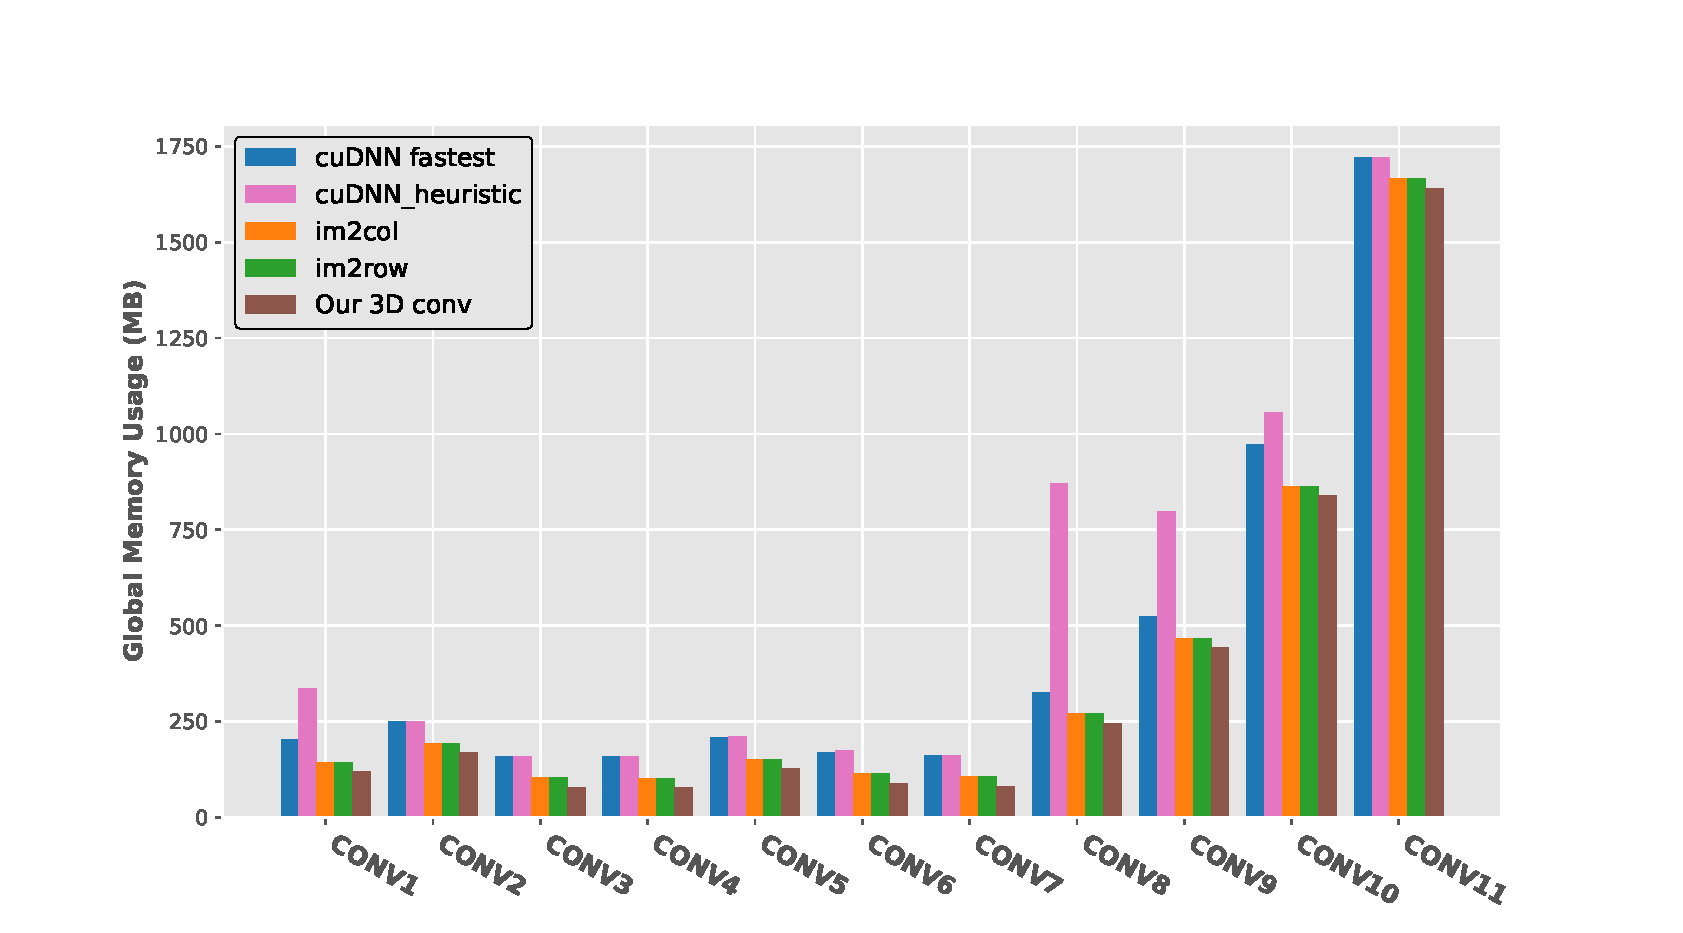
\includegraphics[width=\columnwidth,height=6cm]{./figure/mem3d_1.eps}
%	\label{fig:3dmemk40m}}
%\hspace{0em}
%\subfloat[]{\includegraphics[width=\columnwidth,height=6cm]{./figure/mem3d_1_rtx2080.eps}
%	\label{fig:3dmemrtx2080}}
%
%\caption{Global memory usage for five implementations. Left figure demonstrates the result on Tesla K40m and right figure demonstrates the result on RTX 2080 Ti.}
%\label{fig:3dmem}
%\end{figure*}

We collect configurations of the convolutional layers using depth-wise convolution from three popular mobile CNN models,
namely, MobileNetv2, ShuffleNetv2 and EfficientNet.
Then, we set the number of the batch size to 512 ($I_N=O_N=512$). Other batch sizes demonstrate a similar performance because all tested implementations have a linear scale as the batch size. The exact configuration is presented in Table \ref{tab:3dconvconfigs}.

The speedups are shown in Figure \ref{fig:3druntime}. It is obvious that our implementation performs best in all test cases. We obtain an average speedup of $4.5\times$ and $7.6\times$ for the $3 \times 3$ and $5 \times 5$ filters, respectively. The implicit algorithm is the fastest algorithm in cuDNN in all test cases. It achieves an average speedup of $2.8\times$ and $1.8\times$ for the $3 \times 3$ and $5 \times 5$ filters, respectively. Compared with the fastest algorithm of cuDNN, the proposed approach achieves an average speedup of $1.5\times$, with the maximum speedup reaching $2\times$ for the $3 \times 3$ filter, and an average speedup of $4\times$, with the maximum speedup reaching $4.5\times$ for the $5 \times 5$ filter.

The algorithms of cuDNN except implicit algorithm perform poorly in all test cases and the speedups of these algorithms all below 1. Considering that cuDNN is a closed source, we can only guess that FFT- and Winograd- based algorithms focus on reduction of computation and trades memory performance for speed. Precomp and gemm algorithms need extra memory operations to compute output elements. Moreover, depth-wise convolution is more sensitive to memory performance than multi-channel 2D convolution. Consequently, these algorithms perform poorly on depth-wise convolutions.
 
\begin{figure}
\centering

\subfloat[Memory throughput for the filter of size $3 \times 3$.]{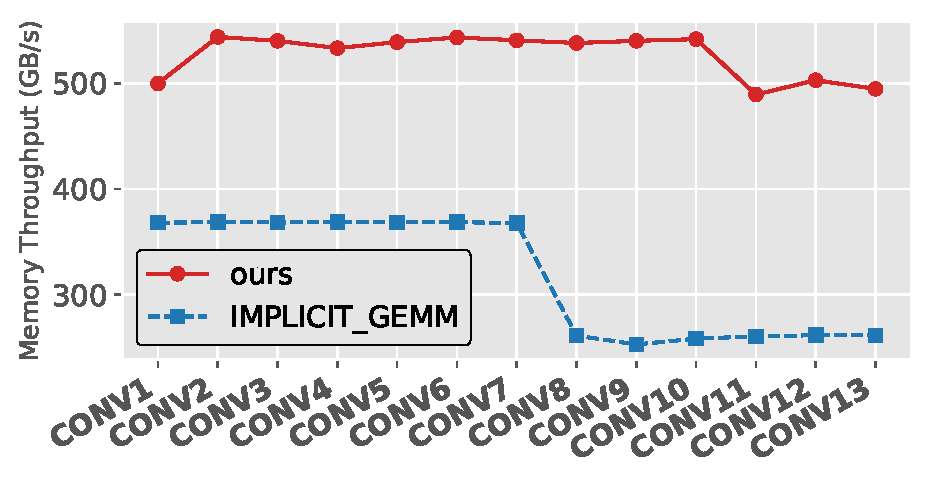
\includegraphics[width=\columnwidth,height=6cm]{./figure/depwisememthroughput.eps}
	\label{fig:depwisememthr}}
\hspace{0em}
\subfloat[Max bandwidth for the filter of size $3 \times 3$.]{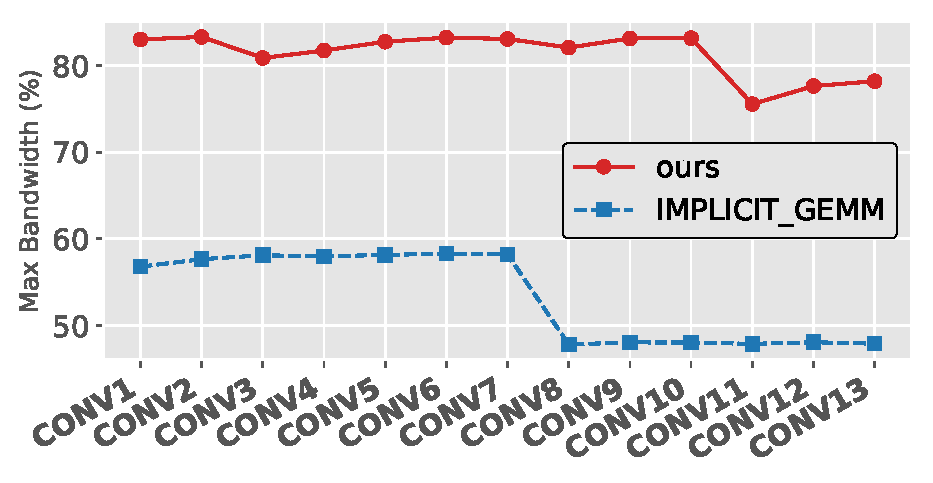
\includegraphics[width=\columnwidth,height=6cm]{./figure/depwisemembandwidth.eps}
	\label{fig:depwisemaxband}}
	
\caption{Memory analysis of cuDNN implicit algorithm and our implementation for the filter of size $3 \times 3$.}
\label{fig:depwisememanaly}
\end{figure}

Figure \ref{fig:depwisememanaly} demonstrates the memory throughput and max bandwidth for our implementation and cuDNN implicit algorithm when convolving with a $3 \times 3$ filter. We can see that our implementation achieves $1.5 times$ memory throughput and max bandwidth compared with the implicit algorithm. This demonstrates that our reuse algorithms can improve the memory performance significantly.
%In contrast to 2D convolutions, the performance gains of 3D convolutions are obtained from two aspects: reduction of the memory transactions of the input data and filters. After loading a filter into the shared memory, we use it to slide over as many images as possible to eliminate the need to load the same filter for each input. Table \ref{tab:3dtrans} lists the number of memory transactions in the four implementations on Tesla K40m. We use the same method used in the 2D convolution to collect the number of memory transactions. Our approach achieves the minimum transaction counts in all tested cases and can reduce the number of memory transactions by a factor of 6.1 and 4.4
%with respect to \emph{cuDNN fastest} with one and three input channels, respectively. Compared with the transaction counts in 2D convolution (Table \ref{tab:2dmemtrans}), that in the 3D convolution has a lower ratio than the other implementations. This phenomenon occurs because in 3D convolutions, each filter needs to slide over all inputs. Hence, we need to load the same filter multiple times. Although we have optimized the use of filters, we still need to load the filters multiple times because the capacity of the shared memory cannot fit the entire
%filters. Consequently, the number of memory transactions increases.

%For 3D convolutions, memory usage is important for the scarce memory storage in GPU. We use \emph{nvidia-smi} command to record the peak GPU device memory usage when the application is running. In this study, we only report the global memory usage for the
%convolutions with one input channel because output data consumes the most memory storage compared with the input and filter data. In addition, changing the number of input channels alone does not change the size of the output data. Therefore, memory usage exhibits only a slight change when we change the number of input channels.

%Figure \ref{fig:3dmem} illustrates the memory usage of the four implementations on two platforms. Our implementation is derived from direct convolution, which does not require extra memory, and therefore consumes the minimum memory storage. GEMM-based implementations (im2col and im2row) first transform the filters into a large matrix before transforming one input into a matrix when performing a matrix multiplication. Therefore, such implementations only need extra memory to store the transformed filters and the transformed input. The most memory consuming
%implementation is cuDNN. Considering that cuDNN is a closed source, we can only guess that this approach improves the performance at the expense of memory usage. The
%memory consumption of our implementation is reduced by 335 MB on average, with the maximum reduction reaching 384 MB with respect to cuDNN fastest. The commonly used
%cuDNN heuristic consumes even more memory than cuDNN fastest. Compared with the cuDNN heuristic, our implementation reduces  memory consumption by 442 MB on average, with the maximum reduction reaching up to 876 MB.

In summary, Both reuse algorithms can significantly improve the memory throughput and max bandwidth, which leads to the improvement of the performance of depth-wise convolutions.  In contrast to cuDNN, which is the state-of-the-art convolution library, our implementation achieves an average speedup of $1.5\times$ and $4\times$ for the $3 \times 3$ and $5 \times 5$ filters, respectively.

